%%
%% Copyright 2007, 2008, 2009 Elsevier Ltd
%%
%% This file is part of the 'Elsarticle Bundle'.
%% ---------------------------------------------
%%
%% It may be distributed under the conditions of the LaTeX Project Public
%% License, either version 1.2 of this license or (at your option) any
%% later version.  The latest version of this license is in
%%    http://www.latex-project.org/lppl.txt
%% and version 1.2 or later is part of all distributions of LaTeX
%% version 1999/12/01 or later.
%%
%% The list of all files belonging to the 'Elsarticle Bundle' is
%% given in the file `manifest.txt'.
%%

%% Template article for Elsevier's document class `elsarticle'
%% with numbered style bibliographic references
%% SP 2008/03/01
%%
%%
%%
%% $Id: podd.tex 1849 2011-05-20 00:39:13Z liyf@itee.uq.edu.au $
%%
%%
\documentclass[preprint,12pt]{elsarticle}

%% Use the option review to obtain double line spacing
%% \documentclass[preprint,review,12pt]{elsarticle}

%% Use the options 1p,twocolumn; 3p; 3p,twocolumn; 5p; or 5p,twocolumn
%% for a journal layout:
%% \documentclass[final,1p,times]{elsarticle}
%% \documentclass[final,1p,times,twocolumn]{elsarticle}
%% \documentclass[final,3p,times]{elsarticle}
%% \documentclass[final,3p,times,twocolumn]{elsarticle}
%% \documentclass[final,5p,times]{elsarticle}
%% \documentclass[final,5p,times,twocolumn]{elsarticle}

%% if you use PostScript figures in your article
%% use the graphics package for simple commands
%% \usepackage{graphics}
%% or use the graphicx package for more complicated commands
%% \usepackage{graphicx}
%% or use the epsfig package if you prefer to use the old commands
%% \usepackage{epsfig}

%% The amssymb package provides various useful mathematical symbols
\usepackage{url}
\usepackage{amsmath}
\usepackage{amssymb}
\usepackage{zed-cm}
\usepackage{graphicx}
\usepackage{dblfloatfix}
\usepackage{boxedminipage}
\usepackage{proof}
%\usepackage{todonotes}

%% The amsthm package provides extended theorem environments
%% \usepackage{amsthm}

%% The lineno packages adds line numbers. Start line numbering with
%% \begin{linenumbers}, end it with \end{linenumbers}. Or switch it on
%% for the whole article with \linenumbers after \end{frontmatter}.
%% \usepackage{lineno}

%% natbib.sty is loaded by default. However, natbib options can be
%% provided with \biboptions{...} command. Following options are
%% valid:

%%   round  -  round parentheses are used (default)
%%   square -  square brackets are used   [option]
%%   curly  -  curly braces are used      {option}
%%   angle  -  angle brackets are used    <option>
%%   semicolon  -  multiple citations separated by semi-colon
%%   colon  - same as semicolon, an earlier confusion
%%   comma  -  separated by comma
%%   numbers-  selects numerical citations
%%   super  -  numerical citations as superscripts
%%   sort   -  sorts multiple citations according to order in ref. list
%%   sort&compress   -  like sort, but also compresses numerical citations
%%   compress - compresses without sorting
%%
%% \biboptions{comma,round}

% \biboptions{}


\journal{Future Generation Computer Systems}

\begin{document}

\begin{frontmatter}

%% Title, authors and addresses

%% use the tnoteref command within \title for footnotes;
%% use the tnotetext command for the associated footnote;
%% use the fnref command within \author or \address for footnotes;
%% use the fntext command for the associated footnote;
%% use the corref command within \author for corresponding author footnotes;
%% use the cortext command for the associated footnote;
%% use the ead command for the email address,
%% and the form \ead[url] for the home page:
%%
%% \title{Title\tnoteref{label1}}
%% \tnotetext[label1]{}
%% \author{Name\corref{cor1}\fnref{label2}}
%% \ead{email address}
%% \ead[url]{home page}
%% \fntext[label2]{}
%% \cortext[cor1]{}
%% \address{Address\fnref{label3}}
%% \fntext[label3]{}

\title{An Ontology-centric Architecture for Extensible Scientific Data Management Systems\tnoteref{t1}}

\tnotetext[t1]{This paper is based on an extended abstract published in the sixth IEEE e-Science Conference, 2010~\cite{podd_escience}.}

%% use optional labels to link authors explicitly to addresses:
%% \author[label1,label2]{<author name>}
%% \address[label1]{<address>}
%% \address[label2]{<address>}

\author[monash]{Yuan-Fang Li}
\ead{yuanfang.li@monash.edu}

\author[uq,csiro]{Gavin Kennedy}
\ead{Gavin.Kennedy@csiro.au}

\author[uq]{Faith Ngoran}
\ead{f.davies@uq.edu.au}

\author[anu]{Philip Wu}
\ead{philip.wu@anu.edu.au}

\author[uq]{Jane Hunter}
\ead{j.hunter@uq.edu.au}

\address[monash]{Clayton School of IT, Monash University}
\address[uq]{School of ITEE, The University of Queensland}
\address[csiro]{High Resolution Plant Phenomics Centre, Canberra}
\address[anu]{The John Curtin School of Medical Research, Australian National University}

\begin{abstract}
Data management has become a critical challenge faced by a wide array of scientific disciplines in which the provision of sound data management is pivotal to the achievements and impact of research projects. Massive and rapidly expanding amounts of data combined with data models that evolve over time contribute to making data management an increasingly challenging task that warrants a new approach. In this paper we present an ontology-centric architecture for data management systems that is extensible and domain independent. In this architecture, the behaviors of domain concepts and objects are captured entirely by ontological entities, around which all data management tasks are carried out. The open and semantic nature of ontology languages also makes this architecture amenable to greater data reuse and interoperability. To evaluate the proposed architecture, we have applied it to the challenge of managing phenomics data.
\end{abstract}

\begin{keyword}
PODD \sep data management systems \sep OWL \sep ontology-centric architecture \sep phenomics \sep bioinformatics
\end{keyword}
\end{frontmatter}

%%
%% Start line numbering here if you want
%%
% \linenumbers

%% main text
\section{Introduction}\label{sec:intro}
Data management is the practice of managing (digital) data and resources, encompassing a wide range of activities including acquisition, storage, retrieval, discovery, access control, publication, integration, curation and archival. For many data-intensive scientific disciplines such as life sciences and bioinformatics, sound data management informs and enables research and has become an indispensable component~\cite{1107503}.

The need for effective data management is, in a large part, due to the fact that massive amounts of digital data are being generated by modern instruments. Furthermore, the fast evolution of technologies/processes and the discovery of new scientific knowledge require flexibility in handling dynamic data and models in data management systems. Among others, there are three core challenges for effective data management in scientific research.

\begin{itemize}
\item The ability to provide a data management service that can manage large quantities of heterogeneous data in multiple formats (text, image, and video) and not be constrained to a finite set of experimental, imaging and measurement platforms or data formats.

\item The ability to support metadata-related services to provide context and structure for data within the data management service to facilitate effective search, query and dissemination.

\item The ability to accommodate evolving and emerging knowledge, technologies and processes.
\end{itemize}

Database systems have traditionally been used successfully to manage research data~\cite{brm2007} in which database schemas are used as domain models to capture attributes and relationships of domain concepts. One implication of the above approach is that domain models need to stay relatively stable as database extension and migration is often an error-prone and laborious task. Consequently, this approach is not suitable for domains where data and model evolution is the norm rather than the exception.

Semantic Web ontology languages such as RDF Schema and OWL possess expressive, rigorously-defined semantics and non-ambiguous syntaxes. Moreover, they have been designed to be open and extensible and to support knowledge and data exchange on the Web~\cite{linkeddata,aue07dbpedia}. These intrinsic characteristics make them an ideal conceptual platform on which a flexible scientific data management system can be built.

The ontology language OWL is being widely used as a modeling language in a number of domains, notably in life sciences and biotechnology~\cite{journals/bib/RuttenbergRSM09,citeulike:1882392,citeulike:212874}, due to its expressivity and extensibility. There is also an increasing number of tools to support tasks including reasoning, querying and visualization, making it a viable option for the modeling and representation of scientific domain concepts.

Moreover, with the rapid progression of Semantic Web-based data integration through the community-driven Linked Data project~\cite{citeulike:5008761}, it is advantageous for data management systems to support Semantic Web languages and standards natively to benefit from the rapidly expanding, integrated open datasets. 

In this paper, we present our work in designing PODD (Phenomics Ontology Driven Data Management), an extensible, domain-agnostic architecture for scientific data management that uses an ontology-centric approach. In our architecture, we support data and model changes through ontology-based domain modeling. Ontologies are at the core of the system - the behaviors of abstract domain concepts and concrete domain objects are entirely defined by ontological vocabularies. Logical structure of data is therefore maintained and enforced via ontological definitions and reasoning and not via database schemas and associated constraints. 

The ontology-based domain model is at the core of PODD as it drives the creation, storage, validation, query and search of data and metadata. The object-oriented approach to developing layers of ontology models and the versioning of ontological definitions make PODD highly extensible. 

Based on the ontology-centric architecture, we have developed the PODD repository~\cite{podd_icadl} to meet the above challenges facing the Australian phenomics research community. Our aim is to provide efficient and flexible data repository functionality for large-scale phenomics research data, and to provide a mechanism for maintaining structured and precise metadata around the raw data so that the combined data/metadata can be stored, distributed and published in a reusable fashion. 

We would like to emphasize that although the PODD system is geared towards phenomics research, the ontology-centric architecture we propose in this paper is domain-independent and can be applied in any scientific discipline where research output can be conceptually organized in a structured manner. 

The rest of the paper is organized as follows. In Section~\ref{sec:overview} we present related work and give a brief overview of the motivation and goals of the PODD project. Section~\ref{sec:arch} presents the ontology-based architecture for data management systems. In Section~\ref{sec:ont}, we discuss the PODD ontologies in more detail and show how the ontology-based modeling approach is used in the life cycle of repository concepts and objects. 
%In this architecture, we rely heavily on ontology reasoning for validation and other purposes. 
Ontology versioning and dynamic composition is central to the support of co-evolution of knowledge and data, and to the maintenance of knowledge and data consistency. The semantics of these operations are formally defined in Section~\ref{sec:spec} using first-order logic and set theory. In Section~\ref{sec:sys}, we describe the implementation of the PODD data management system and evaluation results to date. Finally, Section~\ref{sec:concl} concludes the paper and identifies future directions.

\section{Related Work, Motivation \& Goals}\label{sec:overview}
Over the years attempts have been made to develop content repository systems and architectures to meet institutional and personal data management needs. In this section, we introduce a number of such systems and architectures. With this survey of related work, we present the motivation behind the ontology-centric architecture and the goals we wish to achieve with the PODD data management system.

\subsection{Scientific Data and Resource Management Systems \& Tools}
Fedora Commons\footnote{\url{http://www.fedora-commons.org/}} is an open-source digital resource management system based on the principles of modularity, interoperability and extensibility. In Fedora Commons, abstract concepts are defined as models, on which inter-relationships and behaviors can be further defined. Data in Fedora Commons repositories are represented as objects, which contain datastreams that store either metadata or data. Fedora Commons makes heavy use of Semantic Web technologies through the use of common RDF vocabularies and the integration with the Mulgara triple store\footnote{\url{http://www.mulgara.org/}}, which can be used for metadata storage and queried using SPARQL\footnote{\url{http://www.w3.org/TR/rdf-sparql-query/}}. 

Apache Jackrabbit\footnote{\url{http://jackrabbit.apache.org/}} is an open-source implementation of the Content Repository for Java Technology (JCR) API\footnote{\url{http://jcp.org/en/jsr/detail?id=283}}. In JCR, data is stored in a tree of nodes, which can hold properties of arbitrary values, which is conceptually similar to Fedora Commons. Types can be defined on nodes to place certain restrictions on them.

Fedora Commons and JCR both support fairly basic mechanisms for defining object relationships. Hence, they are usually used as the underlying repository solution on which complex data and document management systems are built. These systems include the National Science Digital Library (NSDL)\footnote{\url{http://nsdl.org/}}, PLoS ONE\footnote{\url{http://www.plosone.org/}}, Biodiversity Heritage Library\footnote{\url{http://www.biodiversitylibrary.org/}} and Fez\footnote{\url{http://fez.library.uq.edu.au/}}, among others. In contrast to our ontology-centric approach, these systems are reliant upon database schemas as their domain models.

%Data management systems have also been developed to support a number of scientific disciplines including high-energy physics, bioinformatics and Earth observation~\cite{652836}.

Bioinformatics Resource Manager (BRM)~\cite{brm2007} is one example of client-server style data management software for bioinformatics research. The client software is installed on users' computers to access (microarray and proteomic) resources stored on BRM server in a PostgreSQL relational database. The BRM server supports data acquisition from external sources such as NCBI~\cite{ncbi} and UniProt~\cite{citeulike:503151}. It also supports annotation using public datasets and connectivity to analytics tools. Data in BRM is stored under the \emph{Project} concept and is mostly flat, i.e., it does not support hierarchical domain concepts such as investigation and publication. %SciPort~\cite{1326001} is a peer-to-peer based platform for scientific data integration.

ArrayExpress~\cite{citeulike:3501974} is a public database of microarray gene expression data. Its three components, the Repository, the Warehouse and the Atlas, contains a large amount of data about functional genomics experiments, gene expression profiles and summaries and analytical tools for gene expressions across experiments and biological conditions. ArrayExpress is built on top of a number of relational databases. Recently, an Experimental Factor Ontology (EFO), a controlled vocabulary of diseases, multi-species anatomy, compounds and cell-type terms has been developed to support the annotation of data in ArrayExpress. The EFO ontology contains mapping to other ontologies including the Disease Ontology\footnote{\url{http://diseaseontology.sourceforge.net/}}, the NCI Thesaurus\footnote{\url{http://ncit.nci.nih.gov/}} and the Cell Type ontology\footnote{\url{http://lists.sourceforge.net/lists/listinfo/obo-cell-type}}.

Besides data management systems, grid-based middleware systems have also been developed to provide distributed storage solutions. Such systems include the Storage Resource Broker (SRB)~\cite{783165} and the CERN Data Grid~\cite{652836} and other systems that make use of Globus\footnote{\url{http://www.globus.org/}} middleware. These systems store data in a distributed environment and usually support authentication, replication, redundancy, etc. However, they are primarily  concerned with data storage and replication and hence do not provide full-fledged data management capabilities. Interested readers are referred to~\cite{565296} for a detailed survey of grid resource management systems. Semantic Grid\footnote{\url{http://www.semanticgrid.org/}} is an extension of Grid technology in which rich metadata is made available to and managed explicitly by applications in the grid. A reference architecture for semantic grid, S-OGSA~\cite{citeulike:1021910}, has been proposed that defines a model and capabilities and mechanisms for the Semantic Grid.

More recently, ontology-based approaches have been taken in VIVO~\cite{vivo10} to model, organize and integrate research activities and researcher profiles in an institutional setting. DOKMS~\cite{Pirro201038} is a distributed, ontology-based knowledge management framework that serves similar purposes as VIVO. DOKMS operates in a P2P environment with desktop clients instead of browsed-based as in VIVO.

\subsection{Domain Modeling in Scientific Research}
A number of specifications and ontologies have been proposed to model scientific research activities. In 2004, the Council for the Central Laboratory of the Research Councils (CCLRC) of UK developed a CCLRC Scientific Metadata Model~\cite{Spallation_metadatamodel} that models \emph{data holdings} in scientific activities in free text. Similar to what we propose here, the CCLCR Scientific Metadata Model logically organises data into objects, whose  definitions are supplied by UML diagrams. The emphasis of this model is on cataloging data, but not integrating data. Compared to this model, our architecture is based on a language with formal semantics. Our architecture also focuses on extensibility and domain independence.

An OWL ontology, EXPO, was developed~\cite{citeulike:3735746} to capture metadata about scientific experiments. EXPO was developed in a top-down manner by extending concepts in the Suggested Upper Merged Ontology (SUMO)\footnote{\url{http://www.ontologyportal.org/}}. Although very comprehensive, these models are quite verbose and consequently are not very suitable as models for developing data management systems.

For a scientific data management system to be effective, models of domain concepts need to be integrated with models of scientific activities and workflows. In biological and particularly 'omics research, a large number of databases have been developed to host a variety of information such as genes (Ensembl\footnote{\url{http://www.ensembl.org/}}), proteins (UniProt\footnote{\url{http://www.uniprot.org/}}), publications (PubMed\footnote{\url{http://www.ncbi.nlm.nih.gov/pubmed/}}) and microarray (GEO\footnote{\url{http://www.ncbi.nlm.nih.gov/geo/}}). These databases are generally characterized by the fact that they specialize in a particular kind of data (protein sequences, publications, etc.) and that their conceptual domain models, such as genes~\cite{citeulike:212874} and microarray experiments~\cite{citeulike:151946}, are well understood. However, models of biological and clinical investigations are less well understood.

The Ontology for Biomedical Investigations (OBI)\footnote{\url{http://purl.obolibrary.org/obo/obi}} is an ongoing effort aimed at developing an integrative ontology for biological and clinical investigations. It takes a top-down approach by reusing high-level, abstract concepts from other ontologies. OBI includes 2,600+ OWL classes and 10,000+ axioms (in the import closure of the OBI ontology). Although OBI is very comprehensive, its size and complexity makes reasoning and querying of OBI-based ontologies and RDF graphs computationally expensive and time consuming, making it impractical as a domain model for data management systems where such reasoning may need to be performed repeatedly.

The Functional Genomics Experiment Model (FuGe)~\cite{citeulike:1756058} is an extensible modeling framework for high-throughput functional genomics experiments, aimed at improving the consistency and efficiency of experimental data modeling for the molecular biology research community. Centered around the concept of experiments, it encompasses domain concepts such as \emph{Protocol}, \emph{Sample} and \emph{Data}. FuGe is developed using UML from which XML Schemas and database definitions are derived. The FuGe model not only covers concepts specific to scientific research such as \emph{Analysis}, \emph{Sequence} and \emph{Investigation}; it also defines commonly used concepts such as \emph{Audit}, \emph{Reference} and \emph{Measurement}. Extensions in FuGe are defined through inheritance of UML classes.

FuGe provides \emph{extension points} to support the addition of technology-specific data formats~\cite{citeulike:4540763}. The \emph{Audit} package in FuGe provides experimental versioning support to track changes to data objects. However, it has not yet been defined how models can be versioned~\cite{citeulike:4540763}.

Observations and Measurements is an International Standardization effort (ISO/PRF 19156)\footnote{\url{http://www.iso.org/iso/catalogue_detail.htm?csnumber=32574}} under development that defines a conceptual model and encoding for observations and measurements for geographic information systems (GIS). This standard, is a core part of the Open Geospatial Consortium (OGC) Sensor Web Enablement that aims at providing annotations for sensor data. A core component of this standard is the Observation Schema, which defines a set of core features for an observation, including feature of interest, observed property, observation procedure and result. This schema takes a user-centric point of view, emphasizing on the meaning of the observation. An XML Schema\footnote{\url{http://schemas.opengis.net/om/2.0/}} and an OWL implementation\footnote{\url{https://www.seegrid.csiro.au/subversion/xmml/ontologies/Ogc/}} have been developed to formally define this schema.

\subsection{The Phenomics Domain as a Motivation for PODD}
Phenomics is a fast-growing, data-intensive discipline in biology with new technologies and processes rapidly emerging and evolving. As a result, its domain model and data management systems must also be able to evolve to handle the complexity, dynamics and scale of the data. 

In phenomics, data is captured by both high- and low-throughput phenotyping devices. The scale of measurement can be from the micro or cellular level, through the level of a single organism, and up to the macro or field level. Imaging, measurement and analysis of organisms on such a large scale produces an enormous amount of data.

In plant phenomics, the objective is to capitalise on emergent technologies to comprehensively measure and study the phenotypes that arise from the plant's genome combined with its development stage, environment and disease factors. New imaging technologies deployed at the High Resolution Plant Phenomics Centre (HRPPC), a node of the Australian Plant Phenomics Facility (APPF), allow for comprehensive imaging and analysis of plant morphology and function. Through visual imaging plant characteristics such as leaf area, biomass, structure and damage can be identified and measured. Far infrared imaging allows profiles of leaf temperature and water usage to be obtained. Near infrared imaging can measure actual water content in plant tissue and soil substrates. FTIR and hyperspectral imaging determine the presence and distribution of chemical compounds at the cellular level. When combined, these platforms can build up a comprehensive digital profile of a plants phenome, especially when recorded over multiple time points or developmental stages. 

At the HRPPC many plant lines with distinct genotypes can be analyzed in this way to determine their phenotypes. Information on the environmental conditions and treatments of the plant lines are also recorded and available as subsequent metadata and data to support the primary phenotyping data and analysis. This includes data from controlled environment plant growth rooms and cabinets, sensor data from field trials and automated watering and treatment regimes. 

These comprehensive data stacks for a single plant line are then represented in PODD as a combination of metadata and data streams. The PODD domain model describes the data generation platforms (platform), the plant genotypes (genotype), the individual plants that are phenotyped (material), their growth environments (environment) and their treatment regimes (treatment material and treatment). PODD then provides the concept of data objects (data) to wrap data file collections generated by the platforms and to associate with the plant materials. Finally PODD provides analysis objects (analysis) for encapsulating secondary data derived from the analysis of the primary data files. 

Similarly, mouse phenomics research makes use of a large variety of imaging and measurement platforms. The Australian Phenomics Network (APN) utilises PODD for the management of primary phenotyping data and metadata. For example, in mouse histopathology and organ pathology based research, the digital slide scanners are used to scan microscope slides, producing high resolution images of stained organ cross-sections. In clinical pathology, a flow cytometer uses laser diffraction to identify and quantify cell types in mouse blood samples and analyse cell types that are the consequence of an ENU mutation. For each of these platforms metadata on the mutagenized mouse lines are recorded in PODD along with visual recordings of the individual mouse specimens, and summary pathology reports.

In both plant and mouse phenomics the scientific workflows are also incorporated into the ontology as process and protocol objects, allowing researchers accessing the online materials to understand the experimental processes that have been used to derive the phenotypes described.

Because an organism's phenotype is often the product of the organism's genetic makeup, its development stage, disease conditions and its environment, any measurement made against an organism needs to be recorded in the context of these other metadata. Consequently the opportunity exists to create a repository to record the data, the contextual data (metadata) and data classifiers in the form of ontological or structured vocabulary terms. The structured nature of this repository will support both manual and autonomous data discovery as well as provide the infrastructure for data based collaborations with domestic and international research institutions. Currently there are no such integrated systems available. The goals of PODD are to capture, manage, annotate and distribute the data generated by mouse and plant phenomics research activities. 

%\vspace{-6pt}
\section{The Architecture of the Ontology-centric Data Management System}\label{sec:arch}

%\vspace{+4pt}
\subsection{Requirements of Data Management Systems}

For any scientific data management system, a number of requirements need to be satisfied.

\begin{list}{\labelitemi}{\leftmargin=30pt}
\item[\textbf{Data storage and management}] Research activities in data-intensive disciplines such as 'omics often generate huge amounts of data. The ability to efficiently acquire, store and manage large volumes of data is essential.

\item[\textbf{Data contextualization}] Sufficient contextual information needs to be maintained for more effective organization, understanding and discovery of raw data. Contextual information includes both conceptual domain models, such as how research activities are organized and carried out; and metadata such as provenance information.

\item[\textbf{Data security}] There are many dimensions to data security, including access control and archival. An effective data management system needs to ensure data security through the use of authentication and authorization and sound versioning and backup solutions. 

\item[\textbf{Data identification and longevity}] In order to support the dissemination of scientific findings, data in the repository needs to be publicly accessible after being published. Hence, a persistent and unique naming scheme is required. Moreover, valuable scientific data also need to be stored in perpetuity.

\item[\textbf{Data reuse and integration}] Contextual information helps to make sense of raw data. Moreover, it also needs to be made discoverable, through mechanisms such as full-text search, faceted browsing and complex query answering, to allow raw data to be integrated and reused.

\item[\textbf{Model extensibility}] A data management system may need to manage a wide variety of data, which may be generated by different software and captured by different platforms. An expressive and extensible domain model is therefore essential to cater for modification, addition and deletion of domain concepts. The data management system also needs to be designed to minimize service disruption when such a model change occurs.
\end{list}

\subsection{The Ontology-centric Architecture For Data Management Systems}\label{sec:arch_desc}
With the data management requirements identified, we design an ontology-centric architecture that satisfies these requirements effectively and efficiently. The most distinguishing characteristic of this architecture is the central role that ontologies play. In our architecture, raw data is not stored in a flat structure but is attached to domain objects organized in a logical, hierarchical system, defined according to the domain model that represents the structure of research activities.

Current document management systems such as Fez typically define a relatively static domain model and hardwire it as relational schemas and foreign key constraints in a custom relational database independent from the underlying repository system. Consequently, the information pertinent to each concrete object is stored in this custom database as well. As stated in the previous section, we find this approach less flexible for dynamic environments where conceptual changes are common.

To effectively support a dynamic conceptual framework, the domain model in the proposed architecture is defined using OWL ontologies, in which: OWL classes represent domain concepts; OWL properties define concept attributes and their relationships; OWL restrictions specify constraints on concepts; and finally, OWL individuals define concrete domain objects where attributes and relationships are defined using OWL assertions. Raw data files are attached to concrete domain objects.

Such a conceptual architecture alleviates the problem of imposing hard relational constraints in a database which is difficult to extend/change.

It is worth noting that referential integrity is not sacrificed in achieving flexibility: ontological reasoning involving relevant concepts and objects is performed before object modification to ensure that all constraints are satisfied.

%Another drawback of existing systems is that there can be only one domain model. When a concept needs to be updated, all the existing objects need to be updated accordingly, which may be undesirable, inappropriate and time-consuming. This is, unfortunately, unavoidable as long as the domain model is defined using database schemas. 

Compared to existing relational data management frameworks, concept changes are naturally supported in our ontology-centric architecture. In our proposed architecture, concepts (schema) and objects (data) are organic entities and their definitions can evolve independently over time. Changes to concept and object definitions are versioned to maintain a complete history. As a result, existing instance objects can remain legitimate when integrity validation is performed as they can still refer to the version of conceptual definition. Details of such operations will be discussed in Section~\ref{sec:spec}.

%\vspace{-8pt}
\begin{figure}[htb]
\centering
\includegraphics[trim = 60mm 30mm 50mm 36mm, clip,height=60mm]{architecture.pdf}
\vspace{-20pt} \caption{A high-level view of the ontology-centric architecture.}\label{fig:arch}
\end{figure}

The high-level design of ontology-centric architecture takes a modular and layered approach, as can be seen in Figure~\ref{fig:arch}. At the foundation is the \textbf{data access layer}, consisting of an underlying repository system, an RDF triple store, a relational database that stores system and user-related information and a full-text search engine. This layer is responsible for low-level tasks supporting the creation, modification and deletion of concepts and objects. The \textbf{business logic layer} in the middle is responsible for managing concepts and objects, such as versioning, object composition and integrity validation. These operations will be further discussed in Section~\ref{sec:op}. The \textbf{security layer} controls access (authentication and authorization) to concepts and objects and guards all operations on them. 

In this architecture, authorization is based on users' access-related attributes, which have two dimensions. Firstly, each user has a system-wide role, such as \emph{registered user} or \emph{system administrator}, which is used to determine access rights across the system. Secondly, a project-wide role, such as \emph{project administrator} and \emph{project observer}, can be assigned so a user can have project-specific access rights. At the top of the stack is the \textbf{interface layer}, where the data management system can be accessed using a number of interfaces such as a Web browser or API calls. 

In developing the ontology-centric architecture, the following design decisions have been made to balance expressivity, flexibility and conceptual clarity. These decisions have been based on a survey of user requirements from scientists within a range of research organizations including the Australian Plant Phenomics Facility (APPF) as well as the Australian Phenomics Network (APN), working on collaborative research projects that involve large scale data and distributed teams.

\begin{itemize}
\item There is a top-level domain concept, called $Project$\footnote{The choice of concept names in the domain ontology is actually irrelevant to the proposed architecture - names such as $Project$ and others are chosen as they are general and representative for a large number of scientific disciplines.}, under which other concepts (such as $Investigation$ and $Material$) reside in a hierarchical manner.

\item Access control (authorization) is defined on the $Project$ level rather than on an individual object level, i.e., a given user will have the same access rights for all objects within a given project.
\item Within a $Project$ hierarchy, objects are in a parent-child relationship in a tree structure such that each child can only have one parent. This ensures that access rights are properly propagated from parent to child and there is no chance of confusion.
\item Additionally, inter-object, many-to-many reference relationships can be defined to enhance flexibility of the architecture as it allows cross referencing between objects to be established.
\item Objects cannot be shared across $Project$s. Instead, objects must be copied from one project and pasted into another one. Such a rule simplifies object management with the elimination of possible side-effects caused by sharing object between projects.

\item There cannot be interference between different versions of a given concept and between objects that are instances of different concept versions.
\end{itemize}

\subsection{Ontology-centric Operations}\label{sec:op}
Versioning, dynamic composition of domain concepts and objects, and ontological reasoning are important operations in the \emph{business logic layer} in Figure~\ref{fig:arch}.  Applied together, these techniques contribute to making this architecture extensible. In this subsection, we describe how these operations are performed on domain concepts and objects (we refer to them as \emph{entities} thereafter). The semantics of these operations are further described in Section~\ref{sec:spec}.

\textbf{Versioning.} As stated previously, all entities are semantically described using ontologies. Each entity (concept and object) maintains a sequence of \emph{versions} of ontologies, from the earliest to the latest, as its semantic definition. Each version contains a unique timestamp and an ontology. A version is created whenever the entity is updated. These versioned ontologies provide a complete change history for each and every entity.
Domain entities refer to each other in their definitions, hence the cross references between versions of ontologies from different entities are also maintained. 

Versioning information is maintained in ontologies with the use of OWL \emph{annotation properties} \texttt{poddModel:versionInfo} and \texttt{poddModel:mapsToVersion}. \texttt{poddModel:versionInfo} annotates an ontology with its own timestamp. \texttt{poddModel:mapsToVersion} annotates the cross references between OWL classes and individuals with the timestamp of the target of the cross reference. Semantics of these annotation properties are further defined in Section~\ref{sec:versioning}.

\textbf{Ontological reasoning.} Before entities can be ingested or updated, their definitions need to be checked to ensure semantic integrity. As ontologies serve as entity definitions, ontological reasoning is performed for integrity checking. Different aspects of integrity are verified, including type correctness and cardinality of entity attributes and associations between entities.

In our architecture, as described in the previous subsection, a domain concept is represented as an OWL class, and a domain object is represented as an OWL individual. Hence, the problem of integrity checking of the concept/object reduces to the verification of consistency of the corresponding OWL class/individual. Such verification tasks are performed by OWL reasoners automatically.

Verification of OWL classes/individuals cannot be performed in isolation as they refer to each other in their definitions. All relevant ontological definitions need to be brought together to form \emph{transient} ontologies. The consistency of such ontologies is verified before the consistency of the OWL class/individual is verified. This is because an inconsistent ontology makes any inference logically invalid. 

\textbf{Dynamic composition.} Transient ontologies are formed by dynamically composing OWL classes and objects in runtime. Dynamic composition is performed in the following scenarios.

\begin{itemize}
\item Before a new object is created, concept ontologies are composed to generate a \emph{template} to drive the rendering of the user input page in HTML. In this case, the latest versions of ontologies of all involved concepts are used for the composition.

\item Similarly, before a new object/concept is saved, the latest versions of relevant concept/object ontologies are composed to verify the consistency of user inputs. The concept may reference other concepts, the corresponding versions (which may not be the latest) of other concepts' ontologies are used in the composition. Effectively, the \emph{closure} of concept ontologies are obtained in the composition.

\item When an existing object is updated, the updated OWL individual ontology is checked against the latest version of the corresponding concept. For other cross referenced objects, the corresponding versions of their ontologies are used in the composition. 
\end{itemize}

From the above discussion it can be seen that reasoning and composition are applied together to maintain entity consistency, and that reasoning tasks are performed on different levels. We refer to these levels as \emph{localities} in Section~\ref{sec:locality}. Initial concept definitions are extracted from base and domain ontologies (described in the next Section). This \emph{bootstrapping} process is further described in Section~\ref{sec:bootstrap}. 

The interactions among these operations are illustrated in the example in Figure~\ref{fig:versions} below. As can be seen here, each of the concepts $C$, $D$ and objects $G$, $H$ and $K$ has a sequence of versions of ontologies ($O_i$'s, $P_j$'s, $Q_k$'s, etc.) and each of these ontologies has a corresponding timestamp ($t_i$'s, $u_j$'s and $v_k$'s). 

Concepts can refer to particular versions of each other's ontologies, as illustrated in Figure~\ref{fig:versions} between concepts $C$ and $D$. Each version of the ontology of an object maps to the corresponding version of the ontology in its concept's definition. For example, ontology version $v_{2}$ of object $G$ refers to version $u_{2}$ in its defining concept $C$. Ontology version $t_{1}$ in object $H$ refers to version $u_{1}$ in the same concept. Hence, they can evolve independently without interference. Similarly, objects can refer to each other's ontologies as well, and the versions of such cross references are maintained as well. Different versions of ontologies of object $K$ refer to different versions of ontologies of objects $G$ and $H$, respectively.

\begin{figure*}[htb]
\centering
\includegraphics[height=90mm]{versions.pdf}

\vspace{-8pt} \caption{A graphical representation of ontology versions and their relationship.}\label{fig:versions}
\end{figure*}

The above three operations are essential to making the proposed architecture extensible and domain-independent. The semantics of these operations are further specified in Section~\ref{sec:spec}.

\section{Ontology-based Domain Modeling}\label{sec:ont}
Domain concepts and objects are described using ontological terms. These terms are defined in the base and domain-specific ontologies that will be described in this section. The \emph{bootstrapping} of concepts using these system ontologies will be further described in Section~\ref{sec:bootstrap}.

As we emphasized previously, the domain model should be flexible enough to accommodate the rapid changes and the dynamic nature of scientific research. In the following subsection, we present the base ontology that we have implemented that defines general vocabularies that are common to many data-intensive disciplines. In Section~\ref{sec:phe_ont}, we present how the base ontology is extended to support phenomics research.

In our modeling approach, we define ontologies on multiple levels. On the base level, the ontology defines domain-independent concepts and their inter-relationships with each other. Based on this base ontology, other more domain-specific ontologies can be developed hierarchically.

\subsection{The Base Domain Ontology}
Inspired by FuGe and OBI, we create the base domain ontology in OWL to define essential concepts in scientific investigations, their attributes and inter-relationships in an object-oriented fashion. As stated in the previous section, concepts are modeled as OWL classes; relationships between concepts and object attributes are modeled as OWL object- and datatype-property assertions. Concrete objects are modeled as OWL individuals.

We define the following design principles for the base ontology.

\begin{itemize}
\item All essential concepts are modeled as subclasses of an abstract top-level OWL class \emph{PODDConcept} that captures common attributes and relationships.

\item All relationships between concepts are captured by domain properties, which can be further divided into two property hierarchies, one for parent-child relationships and the other for reference relationships. Each of the two hierarchies have an abstract top-level property, called \emph{contains} and \emph{refersTo}, respectively. 

\item All parent-child relationships are modeled in a property hierarchy as sub-properties of the abstract property \emph{contains}, and all reference relationships are modeled in another property hierarchy as sub-properties of the abstract property \emph{refersTo}.

\item For each domain concept $C$, one property is defined in each of the above hierarchies with its range defined to be $C$. The domains of such properties are not specified so that they can be used by any applicable domain concept to establish a relationship between them.

\item Class attributes are modeled using OWL restrictions.

\item Essential domain concepts can be sub-classed to provide more specialized and refined information. 

\item To ensure that each object can have at most one parent object, the inverse property of \emph{contains}, \emph{isContainedBy}, is defined so that a max cardinality restriction can be added to the top-level concept \emph{PODDConcept} to enforce it. 

\item We use annotation properties on OWL class definitions and axioms to describe their non-semantic properties. For example, for each OWL subclass axiom, we assign a $weight$ annotation property value to suggest their relative placement in the browser.
\end{itemize}

For an overview, inter-relationships of some of the concepts in the base ontology are shown in Figure~\ref{fig:ont}. For brevity reasons, only parent-child relationships are shown here. The OWL object properties and cross references between classes are not shown. 

\begin{figure*}[htb]
\centering
\includegraphics[width=\textwidth]{top_ont.pdf}
\vspace{-16pt}
\caption{A top-level view of the parent-child relationships between essential concepts.}\label{fig:ont}
\end{figure*}

Some definitions of the top-level constructs are summarized in Figure~\ref{for:concept} in OWL DL syntax. 

On the left-hand side we define the OWL class $PODDConcept$, which is the super class of all the domain concepts in our ontologies. It also defines the property $contains$ and its inverse $isContainedBy$. The expression $\leq 1~ isContainedBy$ ensures that each instance of $PODDConcept$ can only be contained by at most one other object, hence maintaining the single-parent structure in the $contains$ hierarchy.

On the right-hand side we define the concept $Project$ to be a subclass of the conjunction of 4 anonymous class expressions, stating that project must have exactly one project plan, at least one investigation, exactly one start date, and at most one publication date (a project may not have been published).

\vspace{-8pt}
\begin{figure}[htb]
\centering\small
\begin{minipage}[t]{.4\textwidth}
\begin{align*}
&PODDConcept \sqsubseteq \top\\
&\top \sqsubseteq \forall contains.PODDConcept\\
&isContainedBy \sqsubseteq (^-contains)\\
&PODDConcept \sqsubseteq~ \leq 1~ isContainedBy
%&\top \sqsubseteq \forall refersTo PODDConcept\\
%&referencedBy\sqsubseteq (^- refersTo)
\end{align*}
\end{minipage}
\begin{minipage}[t]{.4\textwidth}
\begin{align*}
Project \sqsubseteq~ =~ &1~ hasProjectPlan~\sqcap\\
        & \geq~ 1~ hasInvestigation~\sqcap\\
        &\sqsubseteq~ =~ 1~ hasStartDate~\sqcap\\
        &\sqsubseteq~ \leq~ 1~ hasPublicationDate
\end{align*}
\end{minipage}
%\vspace{-4pt}
\caption{Top-level ontology constructs in the base ontology.}\label{for:concept}
\end{figure}

\subsection{Domain-specific Ontologies}\label{sec:phe_ont}
%As stated before, ontologies such as the Gene Ontology~\cite{citeulike:212874} and Plant Ontology~\cite{citeulike:3008167} are widely used in biomedical research to capture domain knowledge about genes, proteins, sequences and organism phenotypes. In our ontology-centric approach, these ontologies can be used to extend our top-level ontology, add annotations on domain objects to enrich their semantic descriptions and enable cross-application reference and integration.

To describe domain knowledge in phenomics, we extend the base ontology and develop a phenomics ontology by defining additional concepts including \emph{Genotype}, \emph{Gene}, \emph{Phenotype} and \emph{Sequence} as subclasses of \emph{PODDConcept}. Additional OWL object- and datatype-properties are also defined to model the attributes and relationships of these concepts, as shown in Figure~\ref{fig:podd_ont}. Note that \emph{Phenotype} is a subclass of \emph{Observation}. To cater for different domains in phenomics, we can further specialize the phenomics ontology to one for the plant domain and one for the mouse domain. 

\begin{figure}[htb]
%\vspace{-16pt}
\centering
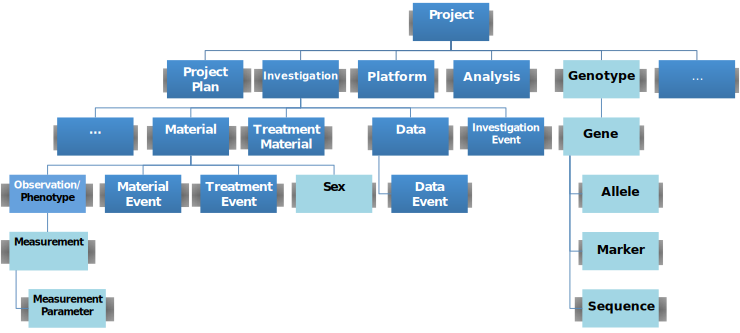
\includegraphics[width=\textwidth]{podd_ont.pdf}
\vspace{-16pt}
\caption{Essential classes in the domain-specific ontology for phenomics.}\label{fig:podd_ont}
\end{figure}

Some important new OWL classes can be seen in Figure~\ref{fig:phe_ont}. Note that in the phenomics ontology we reuse definitions (e.g., $Observation$) from the base ontology to define new concepts. We also refine definitions (e.g., $Project$ and $Material$) in the base ontology with additional restrictions in the phenomics ontology.

\begin{figure}[htb]
\small
\begin{minipage}[t]{.45\textwidth}
\centering
\begin{align*}
Genotype &\sqsubseteq~ PODDConcept\\
         &\sqsubseteq~ \forall hasGene.Gene\\
         &\sqsubseteq~ \leq~ 1~ hasEcotype\\
         &\sqsubseteq~ \leq~ 1~ hasSubspecies
\end{align*}
\end{minipage}
\begin{minipage}[t]{.4\textwidth}
\small\centering
\begin{align*}
Phenotype & \sqsubseteq Observation\\
Project & \sqsubseteq \forall hasGenotype.Genotype\\
Material & \sqsubseteq \forall hasPhenotype.Phenotype~\sqcap\\
         &\quad~ \forall refersToGenotype.Genotype
\end{align*}
\end{minipage}
\caption{Domain-specific OWL definitions.}\label{fig:phe_ont}
\end{figure}

\subsection{Roles of Domain Ontologies in Object Life Cycle}
The base ontology defines essential concepts in a domain-independent fashion. Domain-specific knowledge can be incorporated by extending the base ontology for discipline-specific systems.

As stated in Section~\ref{sec:intro}, the ontology-based domain model is at the center of the whole life cycle of objects. In this subsection, we briefly describe the roles that the domain ontologies perform at various stages of the object life cycle.

\begin{list}{\labelitemi}{\leftmargin=30pt}
\item[\textbf{Ingestion}] When an object is created, its definition is expressed in ontological terms. Such definitions will be used to (a) guide the rendering of object creation interfaces and (b) validate the attributes and inter-object relationships the user has entered before the object is ingested. When an object is ingested, its definitions are stored as RDF assertions.

\item[\textbf{Retrieval \& update}] When an object is retrieved from the repository, its attributes and inter-object relationships are retrieved from its RDF assertions, which are used to drive on-screen rendering. When any value is updated, it is validated and updated in this object's RDF assertions.

\item[\textbf{Query \& search}] An object's assertions will be stored in an RDF triple store, which can be queried using the SPARQL query language. Similarly, RDF assertions are indexed to provide functionalities such as full-text search and faceted browsing. 

\item[\textbf{Publication \& export}] When an object is published or exported, its metadata, in RDF, will be retrieved and exported.
\end{list}

\subsection{Vocabulary Reuse}
Ontologies in the Semantic Web are designed to be shared, reusable and reused. A large number of ontologies and associated concrete RDF data have been developed in the Linked Data project~\cite{citeulike:5008761}. Hence, it is beneficial, and advisable to reuse vocabularies whenever possible.

In our architecture, external vocabularies are used as \emph{annotations} on concepts and objects while local ontologies define their basic semantics. Such an approach maintains semantic integrity of the domain while maximizing knowledge reuse and integration.

\section{Knowledge \& Data Co-evolution: Dynamic Ontology Composition \& Versioning}\label{sec:spec}

As stated previously, high extensibility is an important design goal for our ontology-centric architecture. A prerequisite to this goal is that the knowledge and the data described by the knowledge are able to evolve independently. Moreover, to ensure consistency, it is also necessary to perform integrity consistency checks on certain operations that modify the state of the system, knowledge or data.

The architecture proposed here achieves these two goals through the combination of concepts and objects \emph{versioning} and \emph{dynamic composition}. In this section, we formally define their definitions and show how we employ them in a declarative fashion.

%\subsection{Concepts, objects \& their ontological definitions}
As can be seen in Figures~\ref{fig:ont} - \ref{fig:phe_ont}, the semantics of the domain is described by a number of \emph{concepts}. Concrete \emph{objects}, defined by the concepts, represent real-world metadata entities that encapsulate raw data. The attributes and relationships between concepts and objects are entirely defined by ontologies\footnote{Note that the interpretation of \emph{ontology} in this section is slightly relaxed to include both OWL and RDF definitions.}. The versioning, reasoning and composition operations are defined over these ontologies. In Section~\ref{sec:op} we introduced these operations. In this section, we give formal definitions and present their semantics.

\subsection{Notations}
Here we define the notations that will be used in the rest of this section.
\begin{itemize}
\item Concepts and objects: $A$, $B$, $C$,
%\item Definitions of concepts and objects: $\mathcal{O}$, $\mathcal{P}$, $\mathcal{Q}$,
\item The ontology datatype: $\bbold{O}$, and individual ontologies: $O$, $P$, $Q$, and 
\item The time datatype: $\bbold{T}$, and individual timestamps: $t_1$, $t_2$, $t_3$.
\end{itemize}

\subsection{Ontology Versioning}\label{sec:versioning}
A concept (or object) is defined by a \emph{sequence} of ontologies, ordered by their creation timestamps. Initially the sequence contains only one item, the initial ontology definition for the concept (or object).

Formally, for any given concept $C$, we define its definition $\mathcal{O}_C$ as a non-empty partial function from time $\bbold{T}$ to ontologies $\bbold{O}$.

\begin{align}
\mathcal{O}_C &\colon \bbold{T} \pfun \bbold{O} \mathrm{,~where~~} \#\mathcal{O}_C \neq 0\label{eqn:version}
\end{align}
 
In the above definition, the expression $\#\mathcal{O}_C$ denotes the cardinality of the function $\mathcal{O}_C$. The condition that the cardinality is not 0 ensures that $C$'s definition is non-empty. By this definition, $\bbold{O}_C$, the definition of $C$, is a set of pairs $(time, ontology)$: $\{(t_1, O_1),(t_2,O_2),\ldots,(t_n,O_n)\}$, such that $t_i$'s are unique from each other. Hence, this definition implicitly defines a temporal sequence of ontologies. 

Whenever a concept definition is updated, a new ontology is created and added as the latest version to the sequence $\mathcal{O}_C$. For example, assuming that the current sequence is $\{(t_1, O_1),(t_2,O_2),\ldots,(t_n,O_n)\}$, a modification will add a new ontology $O_{n+1}$ to the sequence, which then becomes $\{(t_1, O_1),(t_2,O_2),\ldots,(t_n,O_n), (t_{n+1},O_{n+1}\}$, and that $t_{i+1} > t_i, \forall 1\leq i\leq n$.

In OWL and RDF, we support such a versioning mechanism through OWL annotation properties. Each version of a concept and object ontology is annotated with a builtin OWL annotation property \texttt{owl:versionInfo}, with the annotation value being the creation time of the ontology. Additionally, each version of an object ontology is also annotated with an annotation property \texttt{poddModel:mapsToVersion}. The value of this annotation is the timestamp of the version of the ontology of the concept that defines this object. We can view these two annotation properties as functions\footnote{For readability reasons we omit namespace names for the annotation properties in the following discussions.}:

\begin{align}
\mathtt{versionInfo}_C &\colon \bbold{O}\pfun \bbold{T} @ \mathtt{versionInfo}_C = (\mathcal{O}_C)^{\sim}\label{eqn:versioninfo}\\
\mathtt{mapsToVersion}_C &\colon \bbold{T}\pfun \bbold{T}\label{eqn:mapsTo}
\end{align}

In Definition~(\ref{eqn:versioninfo}), we define \texttt{versionInfo} as a function from ontologies $\bbold{O}$ to time $\bbold{T}$. It is easy to see that it is the inverse function of $\mathcal{O}$ defined in Definition~(\ref{eqn:version}). %Note that \texttt{versionInfo} is defined as a total function as we require each ontology to have a timestamp.

Definition~(\ref{eqn:mapsTo}) defines \texttt{mapsToVersion} as a function from time $\bbold{T}$ to time $\bbold{T}$. As stated above, for a given object $A$ and a given version of $A$'s ontology $O_A$, the version of the ontology of the corresponding concept $C$, $O_C$, that defines $O_A$ can be obtained by applying the above three functions: 

\begin{align}
O_C = \mathcal{O}_C(\mathtt{mapsToVersion}_A(\mathtt{versionInfo}_A(O_A))) 
\end{align}

With the above versioning mechanism defined, we impose the following additional conditions to ensure that concepts and objects can evolve independently.
\begin{itemize}
\item For any given concept or object, a modification results in a new version of the ontology.
\item For objects, each new version of the ontology maps (\texttt{mapsToVersion}) to the latest version of ontology of its defining concept.
\item For each concept $C_1$,  if it references another concept $C_2$ during modification of its definition, the latest version of the ontology in $C_2$ is used.
\end{itemize}

\subsubsection{Auxiliary Functions}
We also define two auxiliary functions \emph{latest} and \emph{earlierThan}\footnote{The symbol $\power$ in the definitions that follow represents power set.}:

\begin{align}
latest&\colon\power(\bbold{T}\cross\bbold{O})\fun \bbold{O}\text{ where } \forall x\in\power(\bbold{T}\cross\bbold{O});O\in\bbold{O}, \label{eqn:latest}\\
      & latest(x) = O\iff\nonumber \exists t\colon\bbold{T} @ (t,O)\in x \land\nonumber\\
      &\t3\quad~~~ \nexists t_1\colon\bbold{T};O_1\colon\bbold{O} |(t_1,O_1)\in x \land t\leq t_1\nonumber\\
earlierThan&\colon\bbold{T}\cross\power(\bbold{T}\cross\bbold{O})\pfun\power(\bbold{T}\cross\bbold{O})\label{eqn:earlier}\\
      &\text{ where } \forall t\colon\bbold{T};x,y\colon \power(\bbold{T}\cross\bbold{O}) @ earlierThan(t,x) = y \iff\nonumber\\
      &\t1 y\subseteq x\land \nonumber\\
      &\t1 \forall (u,p)\colon x | u < t @ (u,p)\in y\land \nonumber\\
      &\t1 \forall (u,p)\colon y @ u < t\nonumber
%      &\t1 \exists S\colon \power x @ S = \{v\colon\bbold{T};p\colon\bbold{O} | v\leq t @ (v,p)\}\nonumber\\
%      &\t1 O = latest(S)\nonumber
\end{align}

Given a set of pairs from time $\bbold{T}$ to ontologies $\bbold{O}$, the function \emph{latest} returns the latest ontology from this set. This function can be applied to an entity (concept or object) $C$ to return the latest ontology definition: $latest(\mathcal{O}_C)$.

The function \emph{earlierThan} returns the maximal subset of a set of pairs from time $\bbold{T}$ to ontologies $\bbold{O}$ such that the timestamp of each of the pairs in this subset is earlier than the given time point.

\subsection{Dynamic Composition \& Reasoning of Ontologies}\label{sec:locality}
As stated in Section~\ref{sec:arch_desc}, we employ ontological inference to validate the integrity of concept and object definitions. Three types of reasoning tasks are performed for this purpose: ontology consistency checking, OWL class satisfiability checking (for concepts), and OWL individual assertion checking (for objects). Each of the latter two tasks is defined against an ontology $O$\footnote{Note that $O$ is a simplification from the more verbose and precise definition involving domain of interpretation $\Delta^\mathcal{I}$, interpretation function $\mathcal{I}$, the TBox and the ABox. Interested readers are referred to~\cite{basicdl03} for details.}.

\begin{align}
&O\nvDash \bot &\text{[Ontology consistency]}\label{eqn:ont}\\ 
&O\models \lnot \mathtt{C}\sqsubseteq \bot &\text{[class satisfiability]}\label{eqn:sat}\\
&O\models \mathtt{C}(\mathtt{a}) &\text{[individual class assertion]}\label{eqn:assert}
\end{align}

An inconsistent ontology can imply a false formula, hence the consistency of an ontology needs to be maintained. Definition (\ref{eqn:ont}) states that a consistent ontology $O$ should not be a model for the \texttt{owl:Nothing} ($\bot$) class. Definition (\ref{eqn:sat}) states that, with respect to an ontology $O$, for the class \texttt{C} to be consistent, the logical expression that \texttt{C} is not a subclass of $\bot$ must follow from $O$. Similarly, definition (\ref{eqn:assert}) states that for an individual \texttt{a} to be an instance of class \texttt{C}, this logic expression must follow from the ontology $O$.

Versioning of ontologies makes it possible for concepts and objects to evolve independently and it is one of the main reasons of the improved extensibility of the ontology-centric architecture. However, independent co-evolution of concepts and objects makes it a more challenging task to maintain semantic integrity of each of these entities, and hence that of the whole data management system. 

In the rest of this section, we present in detail how ontologies of different concepts/objects are composed dynamically for the inference task. The formal definitions presented here are inspired by works on distributed description logics~\cite{Borgida:2002:DDL:646748.701674} and tiered logic for agents~\cite{DBLP:conf/icaart/CruzC09}.

First of all we introduce the notion of \emph{localities} for reasoning. Locality is an abstract concept: a locality gives scope for ontology reasoning tasks. There is one \emph{local} locality for each entity (concept or object) $C$. As $C$ uniquely represents the entity, we use $C$ to represent its locality as well. There is also a single and unique \emph{global} locality, denoted $\mathbf{G}$. With these notations, we denote an ontology $O_C$ for entity $C$ in its own locality $O_C^C$, $O^A_C$ in the locality of $A$, and simply $O_C$ in the global locality, omitting the superscript $^\mathbf{G}$. 

\subsubsection{Transfer Rules Between Ontology Localities}
The dynamic composition of ontologies requires reasoning on ontologies to be applied for different concepts/objects in their own localities. Moreover, sometimes reasoning needs to be performed on the global level. Ontologies need to be \emph{transferred} semantically for these reasoning tasks. Contexts (localities) and transfer rules for logics have been defined in~\cite{springerlink:10.1007/978-3-642-11819-7_15,buvac95}. Such rules have also been shown to be sound and complete~\cite{buvac95}. Here we adapt these rules for ontologies and show them in Figure~\ref{fig:rules}, where $O$ represents an ontology, $\alpha$, $\beta$ represent the right-hand side boolean expressions in Definitions (\ref{eqn:ont}), (\ref{eqn:sat}) and (\ref{eqn:assert}), and $l$ and $k$ represent localities. The symbol $\models_l$ is to be interpreted as ``shows in the locality $l$'' and $\models$ as ``shows globally''.

\setlength\fboxsep{1pt}
\setlength\fboxrule{0.5pt}
\begin{figure*}[htb]
\centering\small
\fbox{
\begin{minipage}{.98\textwidth}
\hspace{2pt}
\begin{minipage}[t]{.4\textwidth}
\infer[\text{[exit]}]
{O\models \alpha^l}
{O\models_l \alpha}
\end{minipage}
\hspace{72pt}
\begin{minipage}[t]{.3\textwidth}
\infer[\text{[enter]}]
{O\models \alpha^l}
{O\models_l \alpha}
\end{minipage}
\hspace{44pt}
\begin{minipage}[t]{.3\textwidth}
\infer[\text{[K]}]
{O\models (\alpha^l\rightarrow \beta^l)}
{O\models (\alpha\rightarrow \beta)^l}
\end{minipage}
\vspace{16pt}
\linebreak
\begin{minipage}[t]{.4\textwidth}
\infer[\text{[DT]}]
{O\models (\lnot \alpha)^l\iff\lnot (\alpha^l)}
{}
\end{minipage}
\hspace{8pt}
\begin{minipage}[t]{.4\textwidth}
\infer[\text{[Flat]}]
{O\models (\alpha^l)^k \iff \alpha^l}
{}
\end{minipage}
\hspace{16pt}
\begin{minipage}[t]{.4\textwidth}
\infer[\text{[Flat-0]}]
{O\models_l \alpha\iff \alpha^l}
{}
\end{minipage}
\end{minipage}}
\caption{Transfer rules for ontologies between localities.}\label{fig:rules}
\end{figure*}

The (enter) and (exit) rules allow a formula to move up and down between localities. The (K) and (DT) rules ensure that logical connectives are preserved between localities. The (Flat) and (Flat-0) rules preserves truth/falsehood between localities.

\subsubsection{Global Ontology Consistency}
We maintain global consistency by ensuring the intersection of latest ontologies for all concepts is consistent (is not a model for $\bot$, as stated in Definition (\ref{eqn:ont})). This is performed whenever a new concept is added or an existing concept is modified. For any given concept $C$, we \emph{lift} the individual ontology from its own locality to the global locality. %For this reasoning talk, ontologies discussed in this subsection are the latest version for each concept. 

For a data management system in this architecture with $n$ concepts, the overall data model $O^\mathbf{G}$ is the intersection of all ontologies in the global locality:

\begin{align}
O^\mathbf{G} = \bigcap_{i=1}^n O_{C_i} \text{ where } O_{C_i}\colon \mathcal{O}
\end{align}

\subsubsection{Concept Satisfiability}
As stated before, each version of the ontology of a concept defines the concept and possibly references other concepts. Hence, the satisfiability of the concept $C$ (at any given time point) is equivalent to the satisfiability of the corresponding OWL class $\mathtt{C}$ in the ontology $O_C^C$. 

The ontology of any other concept that is referenced in the definition of $C$ needs to be included before the satisfiability of $C$ is checked, as defined in Definition (\ref{eqn:sat}). For any concept $C$, we define a function $closure_C$ that returns the closure of a version of its ontology $O$:

\begin{align}
closure_C&\colon \bbold{O}\fun\bbold{O} @ \forall (O,t)\colon\mathcal{O}_C, closure_C(O) = O_C^C \cap (\bigcap O_{C_i}^C)\label{eqn:aug_ont}\\
    &\t1 \text{for all concepts $C_i$ referenced in $C$ and}\nonumber\\
    &\t1 O_{C_i}^C = closure_{C_i}(latest(earlierThan(t, \mathcal{O}_{C_i})))\nonumber
\end{align}

Let $O_C$ denote a particular version of ontology for $C$ at time point $t$ (i.e., $(t,O_C)\in\mathcal{O}_C$). Let $O^C$ denote the ontology closure for $O_C$. Therefore,

\begin{align}
O^C &= closure_C(O_C)\\
O^C &\models \lnot \mathtt{C} \sqsubseteq \bot\label{eqn:aug_sat}
\end{align}

In Definition (\ref{eqn:aug_ont}), the ontology $O^C$ is defined to be the intersection of $O_C$ and all ontologies of other concepts \emph{lifted} from their own localities and \emph{lowered} to the locality $C$. Note that we apply the two functions in Definitions (\ref{eqn:latest}) and (\ref{eqn:earlier}) to get the latest ontology from $C_i$ that is earlier than $t$, as it does not make sense to reference an ontology defined in the future. $O^C$ then is used to check the concept satisfiability in Definition (\ref{eqn:aug_sat}).

\subsubsection{Individual Class Assertion}
Similar to concept satisfiability, individual class assertions involve the closure of the object ontology, which includes the ontology of the object itself, the ontology closure of the concept and the ontologies of all the other objects referenced in this object. For a given object $A$, we define a function $closure_A$ that returns the closure of a version of its ontology.

\begin{align}
closure_A&\colon \bbold{O}\fun\bbold{O} @ \forall (O,t)\colon\mathcal{O}_A, closure(O) = O_A^A~ \cap\\
    &\t1 closure_C(\mathcal{O}_C(\mathtt{mapsToVersion}(t)))~ \cap\nonumber\\
    &\t1 (\bigcap O_{A_i}^A) \text{, for all objects $A_i$ referenced in $A$ and }\nonumber\\
    &\t3 O_{A_i}^A = closure_{A_i}(latest(earlierThan(t,\mathcal{O}_{A_i})))\nonumber
\end{align}

For object $A$, let $O_A$ denote a particular version of its ontology at time point $t$ (i.e., $(t,O_A)\in\mathcal{O}_A$). Let $C$ be the concept that defines object $A$. Finally, let \texttt{C} denote the OWL class corresponding to concept $C$ and \texttt{a} denote the OWL individual corresponding to $A$. The closure of the ontology $O_A$ and the class assertion are as follows:

\begin{align}
O^A &= closure_A(O_A)\\
O^A &\models \mathtt{C}(\mathtt{a})
\end{align}

\subsection{Bootstrapping Concept Co-evolution}\label{sec:bootstrap}
In Section~\ref{sec:ont} we described the base ontology and a domain-specific ontology for phenomics. In these ontologies, initial definitions (first version of the ontologies) are defined. These ontologies will be decomposed to individual concept ontologies during the system bootstrapping process. Specifically, all \texttt{rdfs:subClassOf} (in the form of $C\sqsubseteq D$) and \texttt{owl:equivalentClass} (in the form of $C\equiv D$) axioms will be grouped by their left-hand side classes. Property and other common definitions will be grouped into a common ontology. After bootstrapping, the concepts will then evolve independently.

\section{The PODD Data Management System}\label{sec:sys}
\subsection{Implementation}
Based on the ontology-centric architecture presented in Section~\ref{sec:arch} and the base ontology presented in Section~\ref{sec:ont} we have implemented the PODD data management system. An instance of the PODD architecture has been deployed in production for the Australian Plant Phenomics Facility (APPF) and can be found at \url{http://podd.plantphenomics.org.au/}. The source code of the PODD repository software has been published in this repository\footnote{\url{http://podd.plantphenomics.org.au/podd/object/poddObject:696}}, demonstrating the versatility of the architecture.

%\vspace{-8pt}
\begin{figure}[htb]
\centering
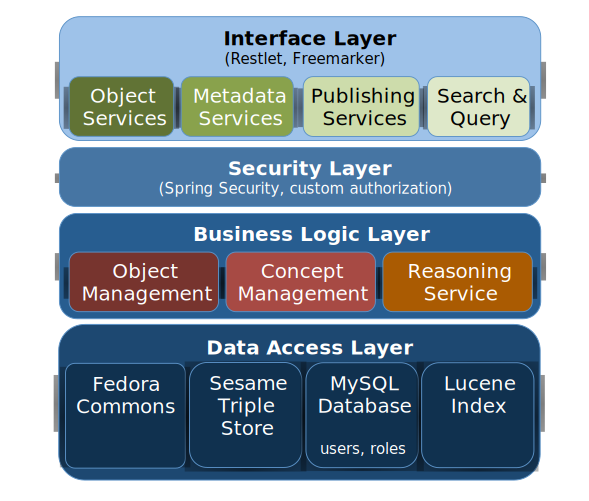
\includegraphics[trim = 60mm 30mm 50mm 24mm, clip,height=72mm]{podd_arch.pdf}

\vspace{-8pt} \caption{The architecture and main components of the PODD system.}\label{fig:podd_arch}
\end{figure}

In developing the PODD system, we chose to employ a number of mature technologies, as can be seen in Figure~\ref{fig:podd_arch}. (1) We use Fedora Commons for the storage and retrieval of domain objects. Together with raw data files, the OWL (for concepts) and RDF (for objects) definitions of each concept and object are stored in a versioned datastream \texttt{PODD}, which is used by the PODD system in various tasks such as object creation, rendering, validation, update and visualization. Moreover, Fedora supports distributed storage through plugins, making it possible to increase the repository storage with demand. (2) We incorporate the Sesame~\cite{conf/iswc02/sesame} triple store to support complex query answering using SPARQL. Sesame \emph{contexts} are used to give scope to the RDF triples for each domain object. As described in Section III, access control needs to be enforced on a per project basis, which also needs to be enforced for query answering in the triple store. By identifying triples of individual objects, we are able to control contexts a user can access through query expansion. (3) We use the Solr\footnote{\url{http://lucene.apache.org/solr/}} open-source search engine platform to provide full-text search and faceted browsing capabilities. Similar to the structure of the Sesame triple store, there is a one-to-one correspondence between domain objects in the repository and the Solr \emph{documents}, the logical indexing units. (4) We use the Pellet~\cite{citeulike:2615678} open-source OWL reasoning engine together with the ontology manipulation library OWL API~\cite{citeulike:6578934} for the inference of ontologies. (5) Lastly, we use a MySQL database to store user and access control related information, as it is orthogonal to other domain concepts.

Although the architecture and the system are based on ontologies, the interface is designed to hide ontology-related complexity from the user and present information in an easy to use manner for all repository functions. For example, Figure~\ref{fig:browser} shows the browser view of a plant phenomics project that investigates leaf stomata in the Arabidopis thaliana model plant. In this view, the objects are shown in a tree-like structure by following parent-child assertions of subproperties of \emph{contains} defined in  the base and domain ontologies.

\begin{figure*}[htb]
\centering
\includegraphics[width=120mm]{browser.png}
\vspace{-8pt} 
\caption{The browser view of a plant project in the PODD repository.}\label{fig:browser}
\end{figure*}

\subsection{Recent Development}
To ease the importing of large amounts of data from existing databases into PODD, we have designed the PODD-TAB format, a simple tab-delimited flat file format that captures essential meta information about raw data. The PODD-TAB format is designed as an intermediate format for users without knowledge of ontologies. Together with the PODD-TAB format, we have developed APIs and tools that enables automatic deposit of data from databases in the Australian Phenomics Network. 

As we stated previously, we store semantic metadata in an RDF triple store. To support advanced users, we have developed a query interface so that users can create complex SPARQL queries to interrogate the repository. SPARQL queries are also used internally by the repository to retrieve information otherwise hard to obtain. For example, for each object, we use a SPARQL query (Figure~\ref{fig:query}) to retrieve all the objects that refer to it. 

\begin{figure}[htb]
\footnotesize\centering
\begin{minipage}{.9\textwidth}
\begin{verbatim}
PREFIX   rdfs:  <http://www.w3.org/2000/01/rdf-schema#>
PREFIX   poddObject:  <http://www.podd.org/object#>
PREFIX   owl:  <http://www.w3.org/2002/07/owl#>
PREFIX   xsd:  <http://www.w3.org/2001/XMLSchema#>
PREFIX   rdf:  <http://www.w3.org/1999/02/22-rdf-syntax-ns#>
PREFIX   poddModel:  <http://www.podd.org/poddModel#>
SELECT DISTINCT ?subject ?type ?label 
WHERE {
    ?subject ?p ?o .
    ?p rdfs:subPropertyOf poddModel:refersTo .
    FILTER (str(?o) = 'http://www.podd.org/object#poddObject:7792')
    ?subject rdf:type ?type .
    ?subject rdfs:label ?label .
    filter (regex(str(?type), 'http://www.podd.org/poddModel#'))
} ORDER BY (?type) (?label)
\end{verbatim}
\end{minipage}
\caption{A SPARQL query to obtain all objects that refer to object \texttt{poddObject:7792}.}\label{fig:query}
\end{figure}

Development has also started on a module to support federated authentication based on the Shibboleth authentication framework\footnote{\url{http://shibboleth.internet2.edu/}}, which allows cross-organization single sign-on and removes the need for users to create a new user account for a Web application. Making use of the Australian Access Federation (AAF)\footnote{\url{http://www.aaf.edu.au/}} infrastructure allows users from AAF-enabled research institutes and universities (more than 60 at the moment) in Australia and New Zealand to access PODD in a seamless manner. The authentication functionality has been implemented and will be integrated in the next major release of PODD.

\subsection{Preliminary Evaluation}
We have started to deploy the PODD system in Australian phenomics research centers including APPF and APN and begun engaging users in the evaluation of the performance, flexibility, usability and scalability of the system. User feedback to date has shown that the system is intuitive and efficient.

It is well known that native RDF triple stores are not yet as efficient as relational database systems, especially in terms of query performance~\cite{10.1109/ICDE.2009.28,Bizer09theberlin}. In the PODD system, we employ a number of approaches to alleviate this problem. Firstly, we give scope to RDF triples of individual objects so a SPARQL query will only be matched against a (potentially very small) subset of the entire triple store, therefore improving query performance. Secondly, we index all RDF datatype property assertions and RDF type assertions in the Solr index to enable faceted searching and filtering. Together with the use of logical operators in search queries, full-text search can be used effectively to perform complex discovery tasks in most cases.

In summary, following the ontology-centric architecture and through the use of mature technologies we have successfully developed PODD, a scalable, extensible data management system. At the same time, data management tasks such as versioning, logical organization of data, authentication \& authorization and discovery are all supported effectively. The PODD system demonstrates the feasibility and practicality of the proposed ontology-centric architecture.

\section{Conclusion}\label{sec:concl}
In this work, our contribution to scientific data management is three-fold: firstly, the proposal of the ontology-centric architecture for developing highly extensible and domain-agnostic data management systems that support the evolution of domain concepts; secondly, the development of a base ontology that defines essential concepts in a domain-independent fashion; and thirdly, the development of a phenomics ontology and the data management system (based on both existing and new technologies) that serves as a validation of the feasibility of the proposed architecture in a virtual laboratory environment.

We have identified a number of future work directions that we would like to pursue:

\begin{itemize}
\item We will investigate the integration with existing domain ontologies such as the Gene Ontology and the Plant Ontology. Potential approaches include using terms defined in these ontologies to annotate metadata objects, and establishing semantic links between concepts/properties through ontology alignment/mapping.

\item We would like to investigate the generalization of the ontology-centric approach and the further abstraction of the PODD base ontology so that the architecture can be applied to other domains including archeology, geological and environmental sciences. 

\item Thus far we have focused on essential functionalities of the PODD system. We will continue the development of the PODD system to provide additional functionalities such as data visualization, data mining and finer-grained representation of repository objects (file contents and metadata) in RDF. 

\item As introduced in Section~\ref{sec:intro}, a huge and growing volume of semantic metadata have been made publicly available as part of the Linked Data project~\cite{citeulike:5008761}. In the Linked Data project, data is organized by application domain into individual RDF datasets. Thus far datasets about a number of domains, including biomedical research, government, geospatial, media and scientific publications, have been created. As of March 2011\footnote{\url{http://www4.wiwiss.fu-berlin.de/lodcloud/state/}}, the Linked Data \emph{cloud} contains more than 28 billion RDF triples and more than 395 million inter-dataset links. This metadata is rich, of high quality and continuously curated. It would be very beneficial for a data management system to reuse this public knowledge.

In our ontology-centric architecture, domain concepts and objects are described using ontological terms in RDF, and such semantic metadata is stored in an RDF triple store. Such a design encourages knowledge integration through the reuse of existing RDF vocabularies. We will investigate a methodology for adding semantic annotation to concepts and objects in the repository. 

We will also investigate approaches to semantically disseminate concepts and objects in our architecture in Linked Data style. As stated above, due to the ontology-centric nature of the architecture, we do not foresee any major difficulties.

\item We will investigate the feasibility of extending the PODD ontology and architecture to support scientific workflow modeling and composition in a virtual laboratory environment, possibly integrating with the widely-used $^{my}$Experiment ecosystem~\cite{DBLP:journals/fgcs/RoureGS09}. 

\item Our current authorization framework is based on user roles,  which are hardcoded and hence inflexible. We will investigate authorization frameworks such as Shibboleth, XACML\footnote{\url{http://www.oasis-open.org/committees/xacml/}} and SemanticAuthz~\cite{MarinPerez201140} and their suitability in our framework. 

\item Last but not least, we will further enhance privacy preservation in the dissemination of repository contents through adoption of fine-grained privacy models such as~\cite{Sun2011348}.
\end{itemize}

\section*{Acknowledgment}
This work is part of a National eResearch Architecture Taskforce (NeAT) project, supported by the Australian National Data Service (ANDS) through the Education Investment Fund (EIF) Super Science Initiative, and the Australian Research Collaboration Service (ARCS) through the National Collaborative Research Infrastructure Strategy Program. 

The authors wish to acknowledge the support of the NCRIS funded Australian Plant Phenomics Facility, including its primary nodes: The High Resolution Plant Phenomics Centre; and The Plant Accelerator. We also wish to acknowledge the support of the NCRIS funded Australian Phenomics Network.

Finally we wish to thank Dr Xavier Sirault and Dr Kai Xu for their assistance in developing the domain models.

\bibliographystyle{elsarticle-num}
\bibliography{all,liyf}

\end{document}

%%
%% End of file `elsarticle-template-num.tex'.
